\newpage
\subsection{Caso d'uso UC 1: Creazione di nuove bolle}
\label{Caso d'uso UC 1: Creazione di nuove bolle}
\begin{figure}[ht]
	\centering
	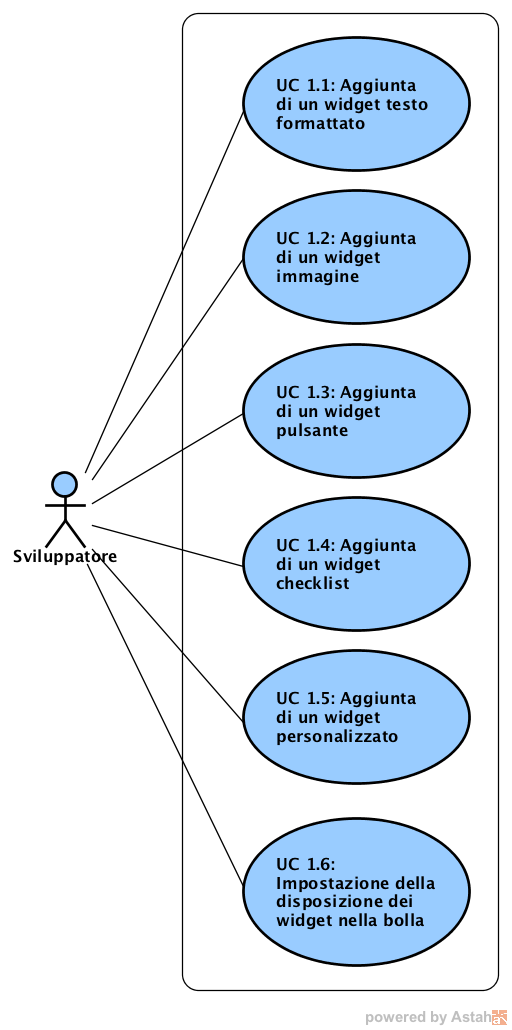
\includegraphics[scale=0.65]{Usecases/img/UC1.png}
	\caption{Caso d'uso UC 1: Creazione di nuove bolle}
\end{figure}

\FloatBarrier
\begin{itemize}
\item \textbf{Attori:} Sviluppatore;
\item \textbf{Descrizione:} Tramite l'\termine{SDK} lo sviluppatore vuole:
	\begin{itemize}
	\item{Aggiunta di un widget testo formattato a una bolla.} 
	\item{Aggiunta di un widget widget immagine a una bolla.}
	\item{Aggiunta di un widget widget bottone a una bolla.}
	\item{Aggiunta di un widget widget checklist a una bolla.}
	\item{Aggiunta di un widget widget personalizzato a una bolla.}
	\item{Impostare la disposizione dei widget nella bolla.}
	\end{itemize} 
\item \textbf{Precondizione:} Lo sviluppatore ha accesso all'\termine{SDK}.
\item \textbf{Postcondizione:} Lo sviluppatore ha creato del codice eseguibile. 
\item \textbf{Scenario principale:}
	\begin{itemize}
	\item{Lo sviluppatore vuole aggiungere a una bolla un widget testo formattato (UC 1.1).}
	\item{Lo sviluppatore vuole aggiungere a una bolla un widget bottone (UC 1.2).}
	\item{Lo sviluppatore vuole aggiungere a una bolla un widget immagine (UC 1.3).}
	\item{Lo sviluppatore vuole aggiungere a una bolla un widget checklist (UC 1.4).}
	\item{Lo sviluppatore vuole aggiungere a una bolla un widget personalizzato (UC 1.5).}
	\item{Lo sviluppatore vuole impostare la disposizione dei wiget nella bolla (UC 1.6).}
	\end{itemize}
\end{itemize}